%%%%%%%%%%%%%%%%%%%%%%%%%%%%%%%%%%%%%%%%%
% Beamer Presentation
% LaTeX Template
% Version 1.0 (10/11/12)
%
% This template has been downloaded from:
% http://www.LaTeXTemplates.com
%
% License:
% CC BY-NC-SA 3.0 (http://creativecommons.org/licenses/by-nc-sa/3.0/)
%
%%%%%%%%%%%%%%%%%%%%%%%%%%%%%%%%%%%%%%%%%

%----------------------------------------------------------------------------------------
%	PACKAGES AND THEMES
%----------------------------------------------------------------------------------------

\documentclass[aspectratio=169]{beamer}

\mode<presentation> {

% The Beamer class comes with a number of default slide themes
% which change the colors and layouts of slides. Below this is a list
% of all the themes, uncomment each in turn to see what they look like.

%\usetheme{default}
%\usetheme{AnnArbor}
%\usetheme{Antibes}
%\usetheme{Bergen}
%\usetheme{Berkeley}
%\usetheme{Berlin}
%\usetheme{Boadilla}
\usetheme{CambridgeUS}
%\usetheme{Copenhagen}
%\usetheme{Darmstadt}
%\usetheme{Dresden}
%\usetheme{Frankfurt}
%\usetheme{Goettingen}
%\usetheme{Hannover}
%\usetheme{Ilmenau}
%\usetheme{JuanLesPins}
%\usetheme{Luebeck}
%\usetheme{Madrid}
%\usetheme{Malmoe}
%\usetheme{Marburg}
%\usetheme{Montpellier}
%\usetheme{PaloAlto}
%\usetheme{Pittsburgh}
%\usetheme{Rochester}
%\usetheme{Singapore}
%\usetheme{Szeged}
%\usetheme{Warsaw}

% As well as themes, the Beamer class has a number of color themes
% for any slide theme. Uncomment each of these in turn to see how it
% changes the colors of your current slide theme.

%\usecolortheme{albatross}
%\usecolortheme{beaver}
%\usecolortheme{beetle}
%\usecolortheme{crane}
%\usecolortheme{dolphin}
%\usecolortheme{dove}
%\usecolortheme{fly}
%\usecolortheme{lily}
%\usecolortheme{orchid}
%\usecolortheme{rose}
%\usecolortheme{seagull}
%\usecolortheme{seahorse}
%\usecolortheme{whale}
%\usecolortheme{wolverine}

%\setbeamertemplate{footline} % To remove the footer line in all slides uncomment this line
%\setbeamertemplate{footline}[page number] % To replace the footer line in all slides with a simple slide count uncomment this line

\setbeamertemplate{navigation symbols}{} % To remove the navigation symbols from the bottom of all slides uncomment this line
}

\usepackage{graphicx} % Allows including images
\usepackage{booktabs} % Allows the use of \toprule, \midrule and \bottomrule in tables
\usepackage{amsmath}
%----------------------------------------------------------------------------------------
%	TITLE PAGE
%----------------------------------------------------------------------------------------

\title[NXTway-GS]{Two wheeled Self-balancing Robot using LEGO NXT Kits} % The short title appears at the bottom of every slide, the full title is only on the title page

\author{S.R.Manikandasriram} % Your name
\institute[IITM] % Your institution as it will appear on the bottom of every slide, may be shorthand to save space
{
Indian Institute of Technology, Madras \\ % Your institution for the title page
\medskip
\textit{srmanikandasriram@gmail.com} % Your email address
}
\date{\today} % Date, can be changed to a custom date

\begin{document}

\begin{frame}
\titlepage % Print the title page as the first slide
\end{frame}

%\begin{frame}
%\frametitle{Overview} % Table of contents slide, comment this block out to remove it
%\tableofcontents % Throughout your presentation, if you choose to use \section{} and %\subsection{} commands, these will automatically be printed on this slide as an overview %of your presentation
%\end{frame}

%----------------------------------------------------------------------------------------
%	PRESENTATION SLIDES
%----------------------------------------------------------------------------------------

%------------------------------------------------
\section{Introduction} % Sections can be created in order to organize your presentation into discrete blocks, all sections and subsections are automatically printed in the table of contents as an overview of the talk
%------------------------------------------------

%\subsection{Subsection Example} % A subsection can be created just before a set of slides with a common theme to further break down your presentation into chunks

\begin{frame}
\frametitle{LEGO 2-Wheel Self-balancing Robot}
\begin{columns}[c] % The "c" option specifies centered vertical alignment while the "t" option is used for top vertical alignment

\column{.45\textwidth} % Left column and width
\textbf{Using}
\begin{enumerate}
\item LEGO Mindstorms NXT 2.0 Kit
\item HiTechnic Gyro Sensor
\item Simulink (with Hardware Support Package for LEGO NXT)
\end{enumerate}

\column{.5\textwidth} % Right column and width
\begin{figure}
	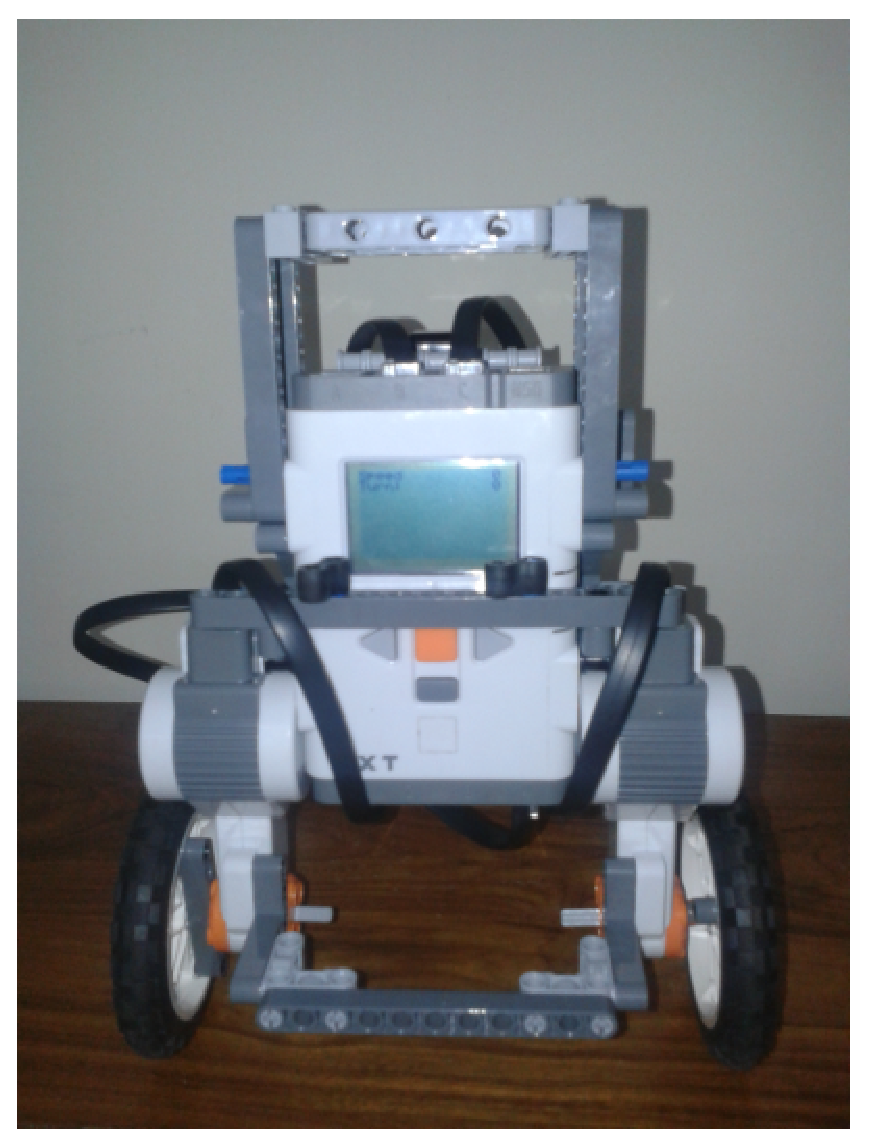
\includegraphics[width=0.5\textwidth]{legoBot.eps}
	\caption{LEGO 2-Wheel Self-Balancing Robot - NXTway-GS}
\end{figure}
\end{columns}
\end{frame}

%------------------------------------------------

\begin{frame}
\frametitle{Mathematical Modelling - Diagram}
\begin{columns}[c]

\column{.45\textwidth}
\begin{figure}
	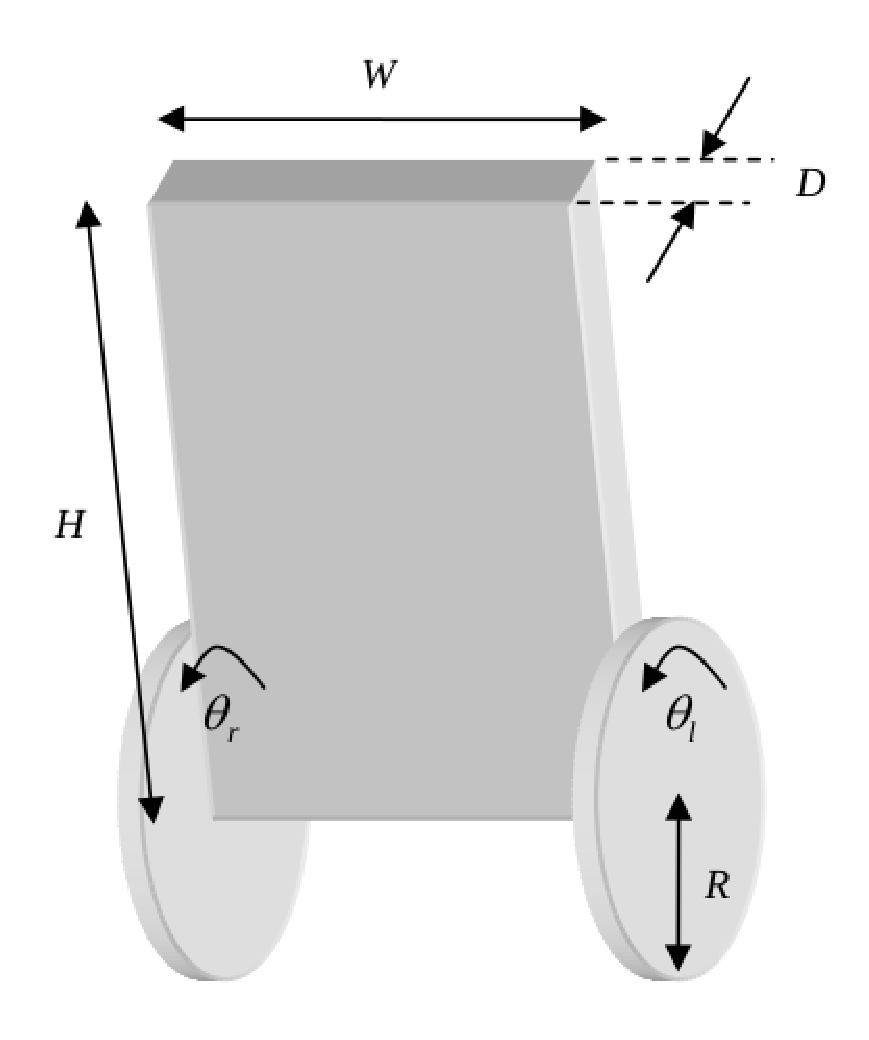
\includegraphics[width=0.5\textwidth]{InvPen.eps}
	\caption	{Two-wheeled Inverted Pendulum model - (clockwise from left) Perspective view, side view and top view}
\end{figure}
\column{.45\textwidth}
\begin{figure}
	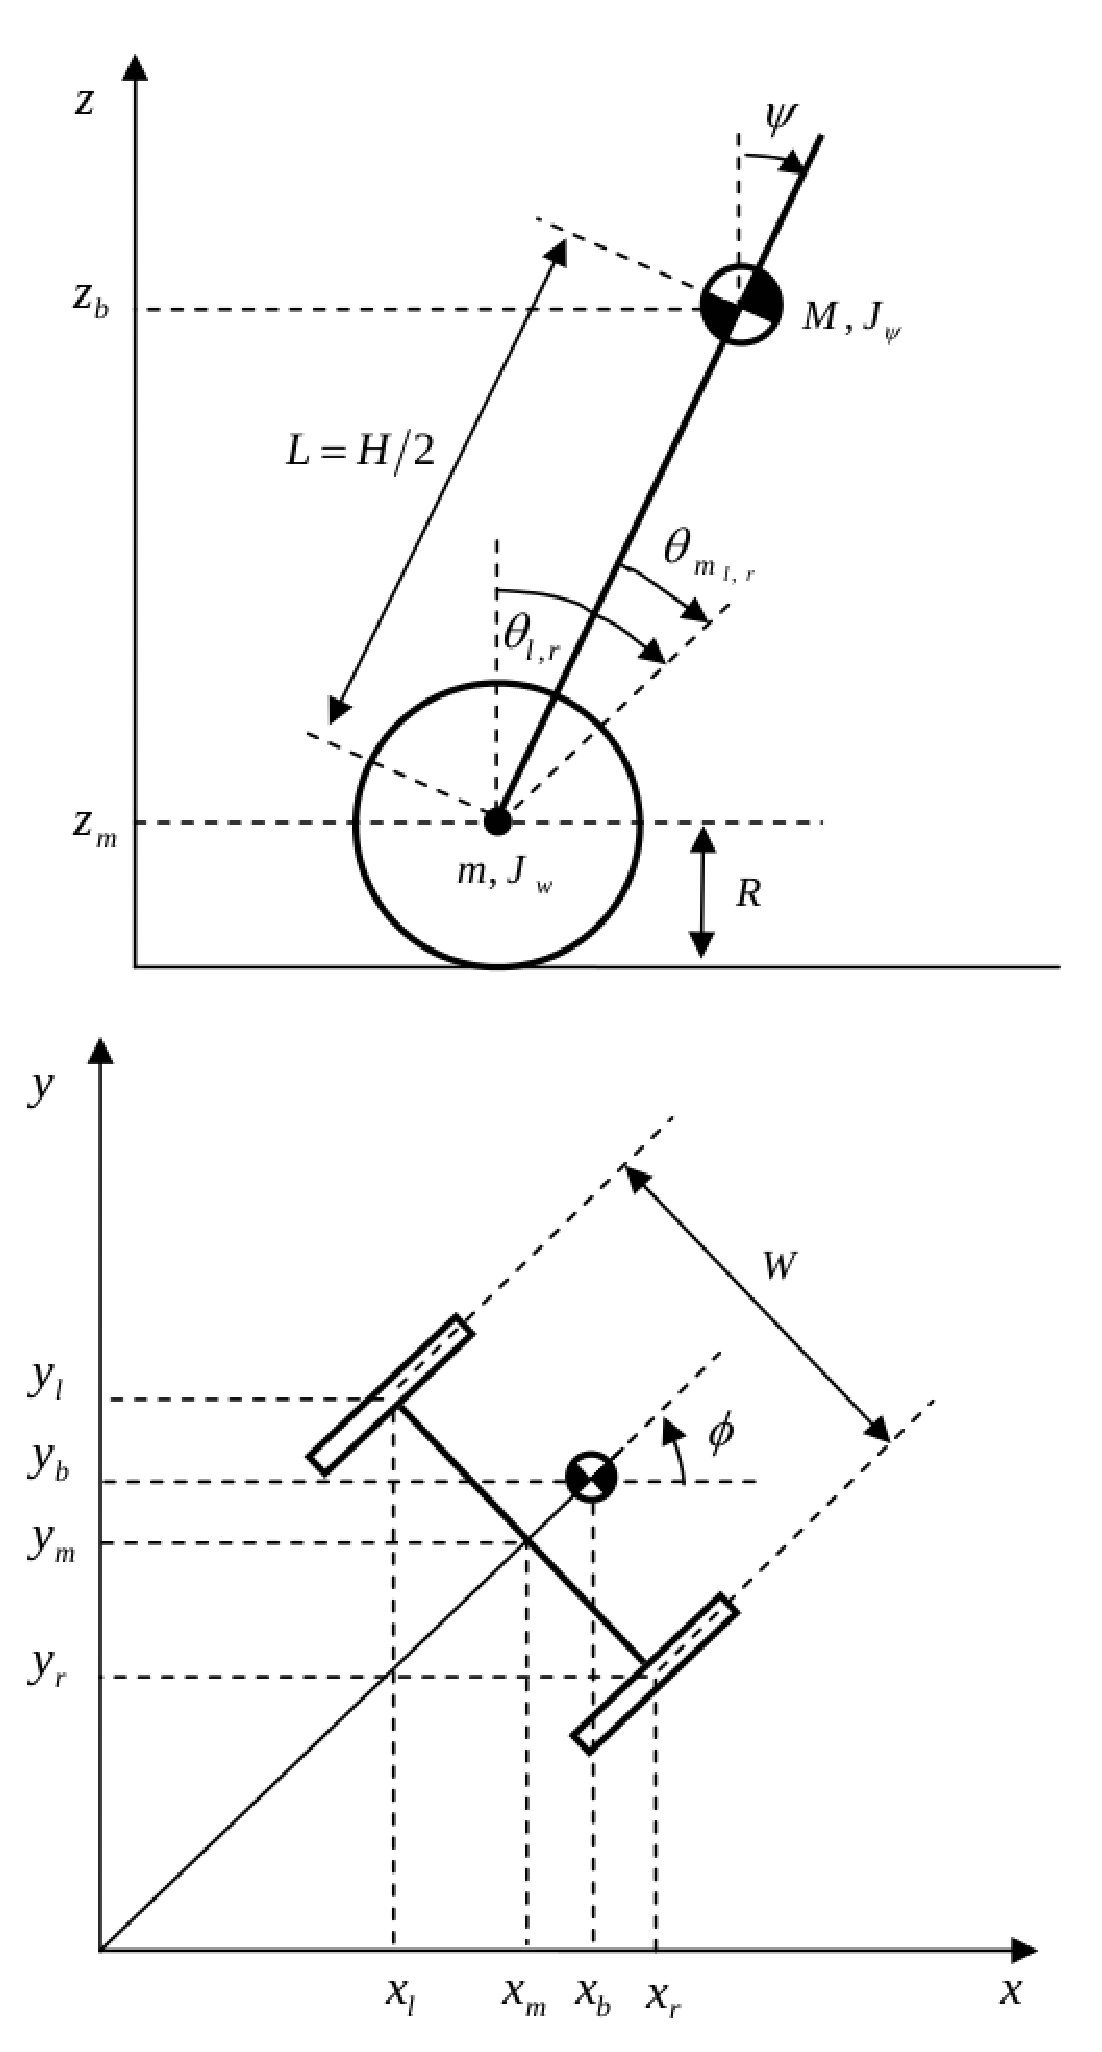
\includegraphics[width=0.5\textwidth]{InvPenSideTop.eps}	
	\caption{Side and plane view of two-wheeled inverted pendulum}
\end{figure}
\end{columns}
\end{frame}

%------------------------------------------------

\begin{frame}
\frametitle{Mathematical Modelling - Equations of Motion}
The equations of motion are derived using Lagrangian dynamics. \\
The Lagrangian takes the form
\begin{displaymath}
L = T - U
\end{displaymath}
The Euler-Lagrange equations of motions for the robot are given by:
\begin{align*}
\frac{d}{dt} \left(\frac{\partial L}{\partial \dot{q_{i}}}\right) - \frac{\partial L}{\partial q_{i}} = Q_{i}\qquad	i = 1,2,\ldots ,n
\end{align*}
where $q = (\theta,\phi,\psi)$ are the generalized coordinates.
\end{frame}

%------------------------------------------------

\begin{frame}
\frametitle{Mathematical Modelling - State Equations of the System}
On solving the Euler-Lagrange equations, a non-linear model of the system is obtained. On linearizing the model about the equilibrium point($\psi=0$) and neglecting second order terms like $\dot{\psi}^2$ and $\dot{\phi}^2$, we obtain:
\begin{align*}
\biggl[(2m+M)R^2+2J_w+2n^2J_m\biggr]\ddot{\theta}
+\left(MLR-2n^2J_m\right)\ddot{\psi} &= F_{\theta} \\
\left(MLR-2n^2J_m\right)\ddot{\theta}+\left(ML^2+J_{\psi}+2n^2J_m\right)\ddot{\psi}-MgL\psi &= F_{\psi} \\
\biggl[\frac{1}{2}mW^2+J_{\phi}+\frac{W^2}{2R^2}\left(J_w+n^2J_m\right)\biggr]\ddot{\phi} &= F_{\phi}
\end{align*}
\end{frame}

%---------------------------------------------------

\begin{frame}
\frametitle{Mathematical Modelling - State Space Representation}
Here, we consider $x_1,x_2$ as states and $u$ as input and thus the state space representation of the linearized model is of the form:
\begin{align*}
\mathbf{\dot{x_1}} &= A_1\mathbf{x_1}+B_1\mathbf{u} \\
\mathbf{\dot{x_2}} &= A_2\mathbf{x_2}+B_2\mathbf{u}
\end{align*}
where,
\begin{displaymath}
\mathbf{x_1}=[\theta,\psi,\dot{\theta},\dot{\psi}]^T, \mathbf{x_2} = [\phi,\dot{\phi}]^T, \mathbf{u} = [v_l,v_r]^T
\end{displaymath}
\end{frame}

%------------------------------------------------------

\begin{frame}
\frametitle{Controller Design}
A Servo (PID type) controller is employed to track the reference signal. An integral gain is inserted into the feedback loop in order to regulate out steady state errors. 

\begin{figure}
    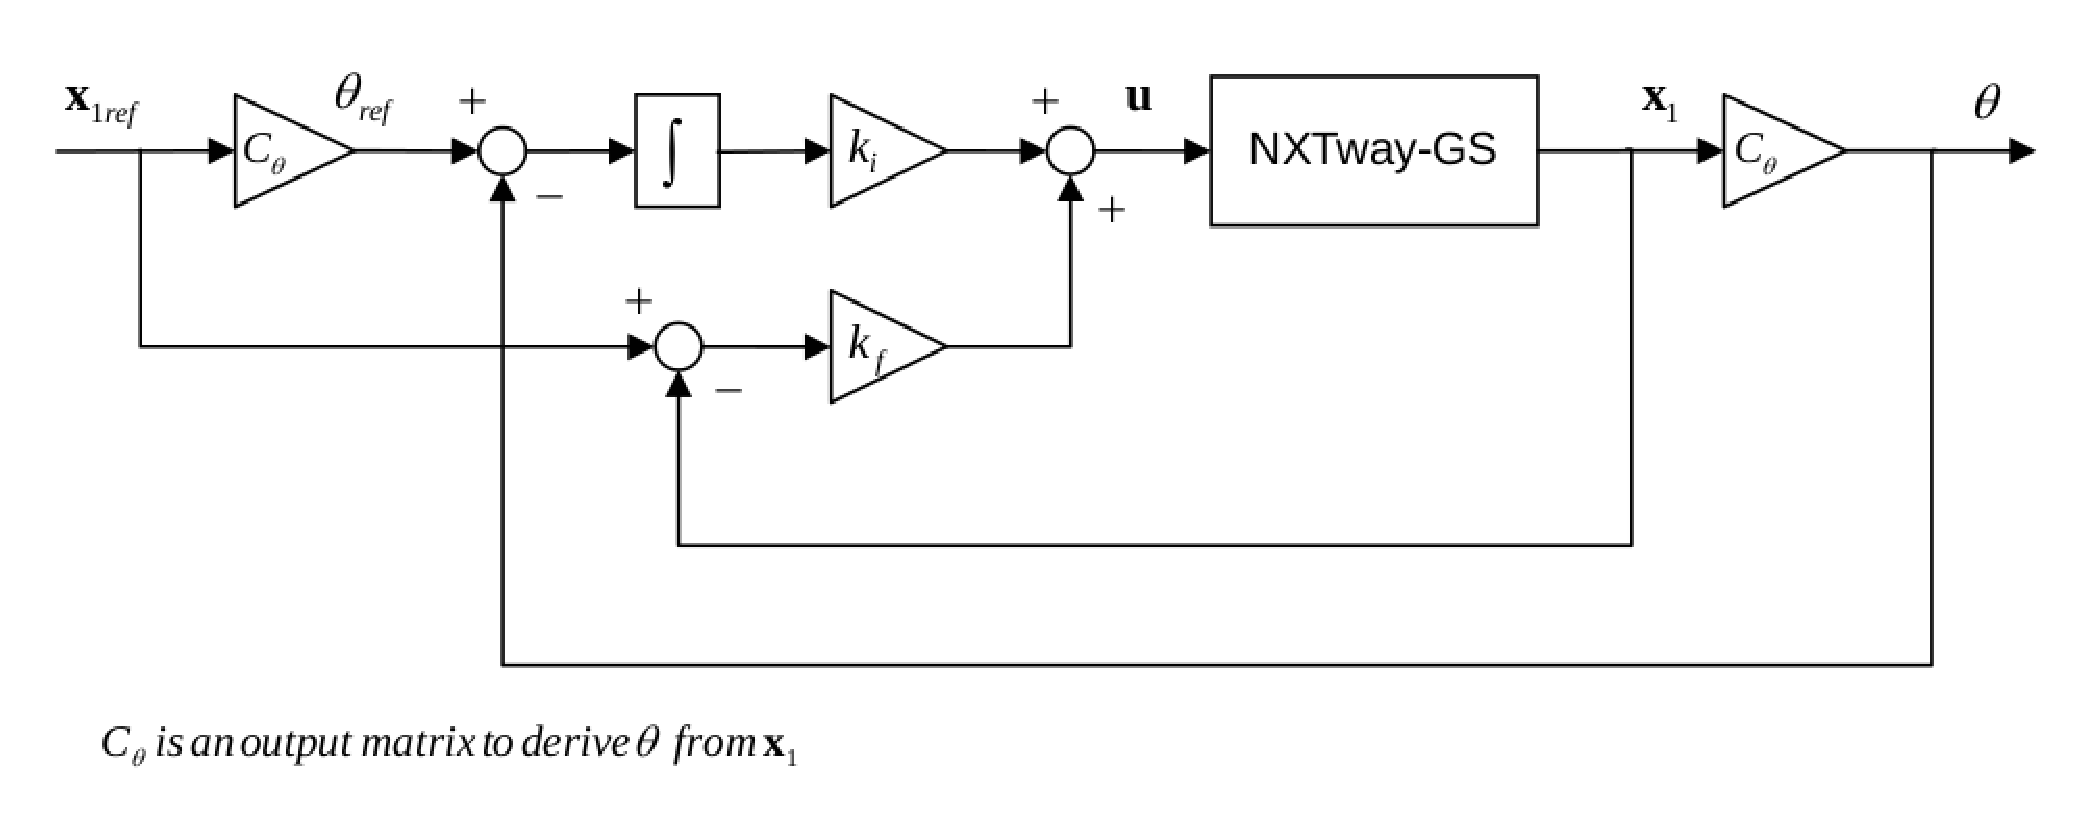
\includegraphics[width=0.85\textwidth]{CtrlBlk.eps}
	\caption{Servo Controller Block diagram}
\end{figure}

\end{frame}

%------------------------------------------------------

\begin{frame}
\frametitle{Controller Design}
Additionally,
\begin{itemize}
\item P control is used for wheel synchronization when moving straight. This is required since two DC motors don't move at the same speed for the same voltage.
\item Rotation is achieved by giving higher power to the left motor
\end{itemize}
\end{frame}

%------------------------------------------------------

\begin{frame}
\frametitle{Simulink Model - NXTway-GS}
\begin{figure}
	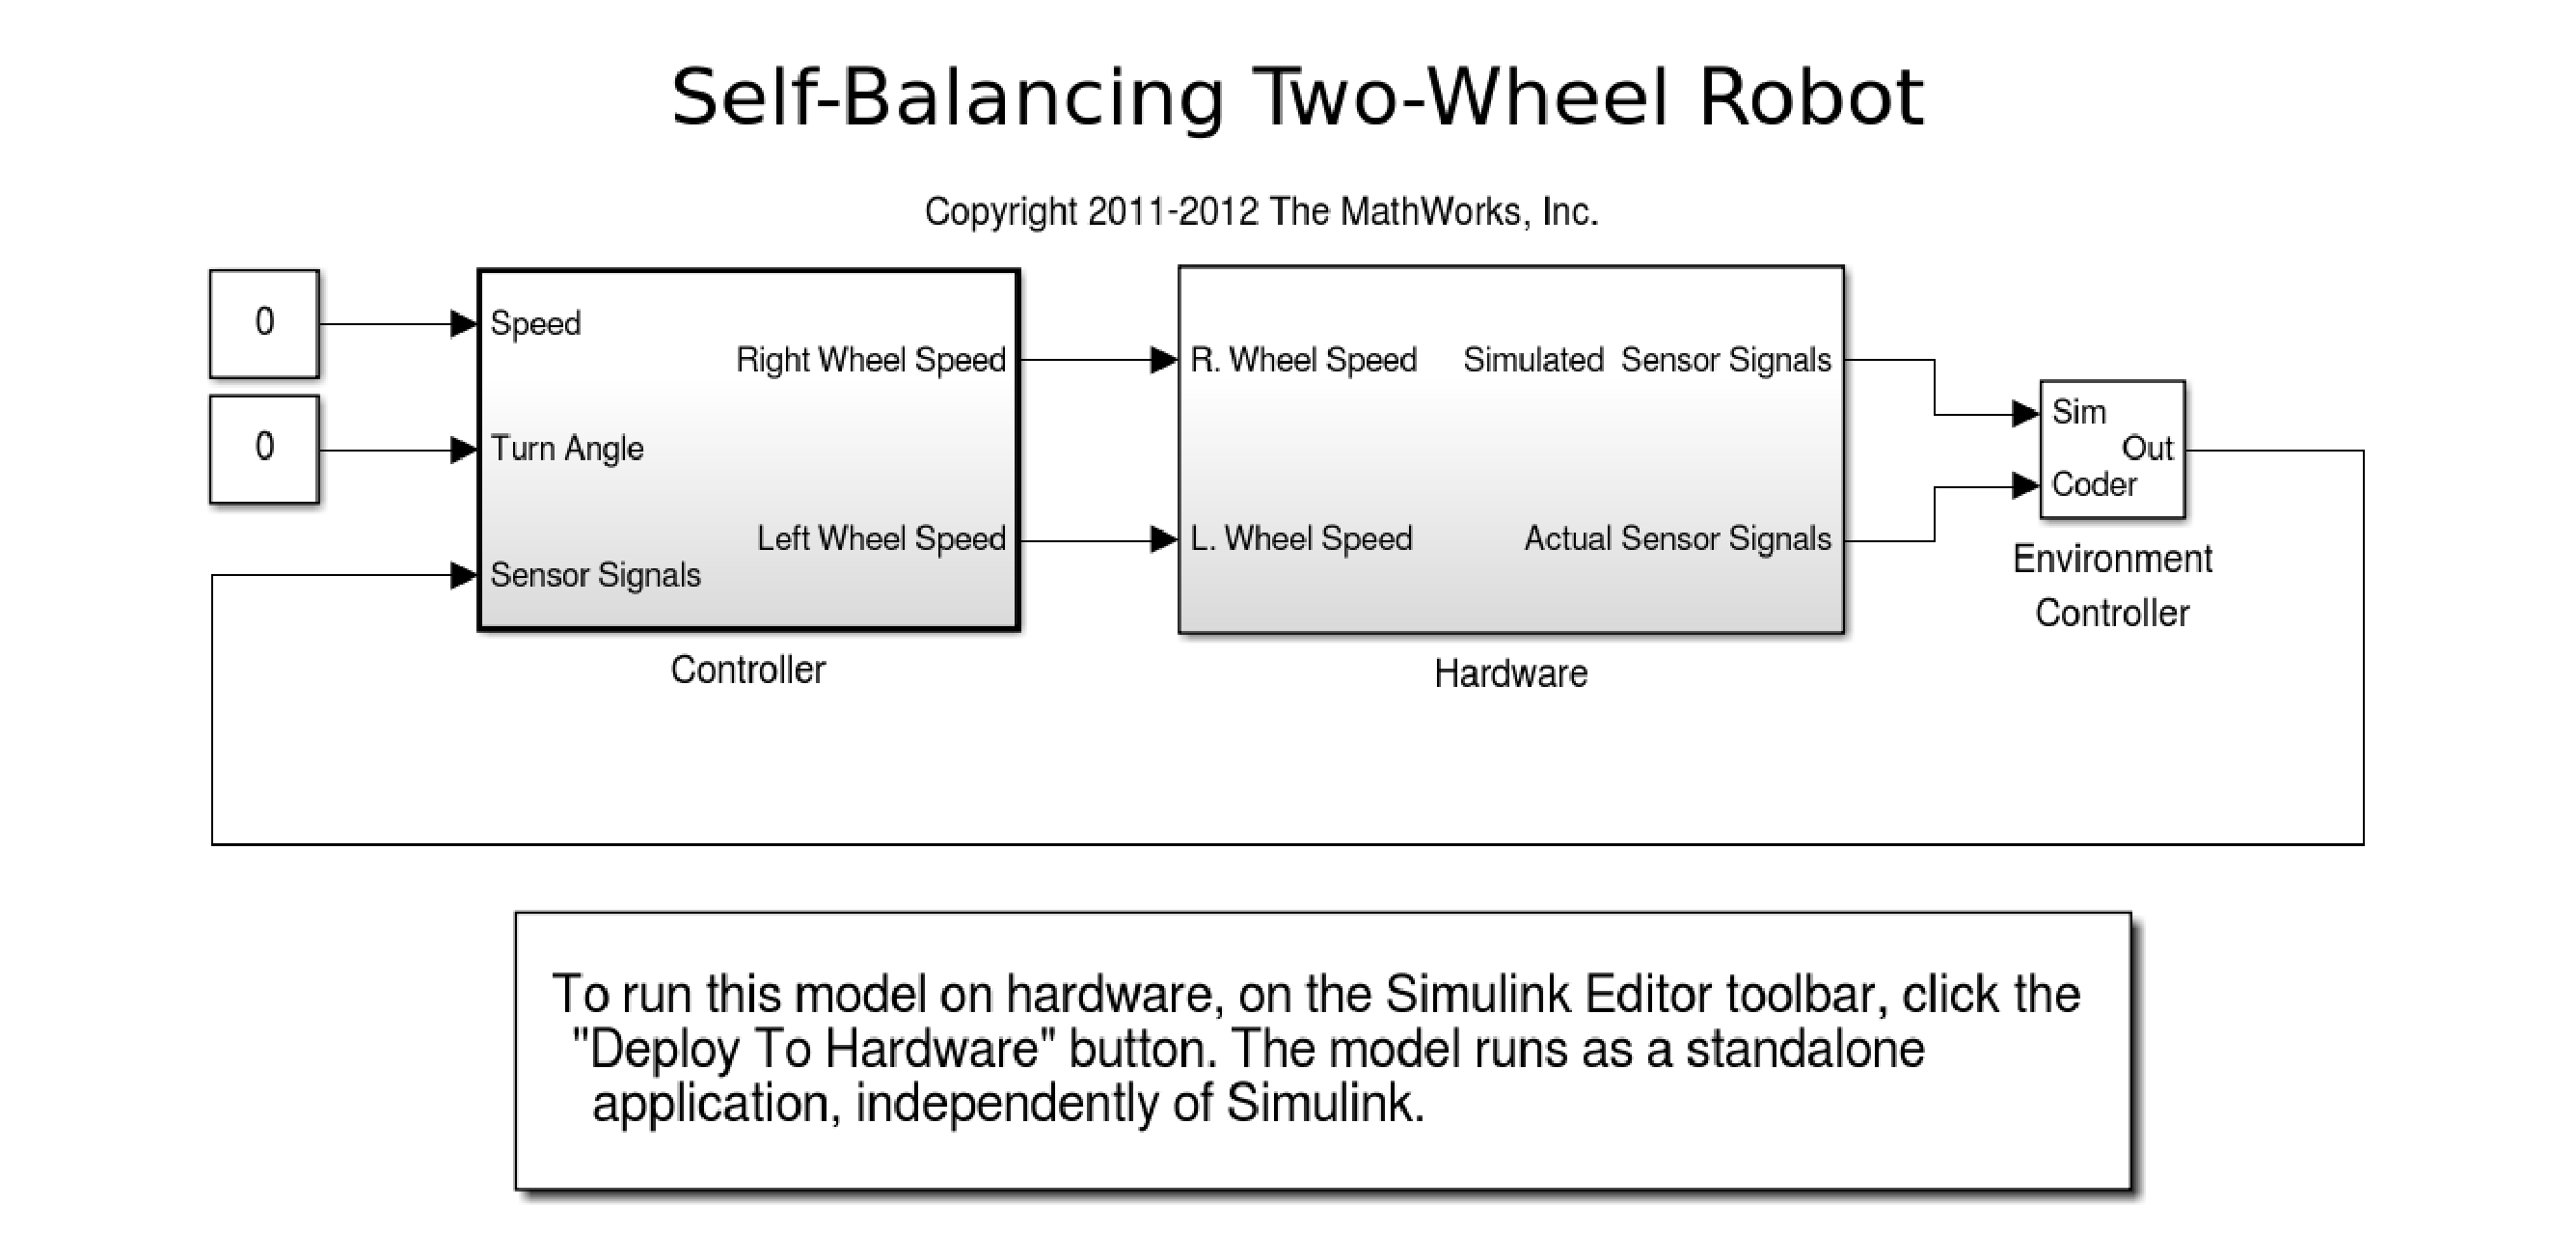
\includegraphics[width=0.5\textwidth]{smdlBot_1.eps}
	\caption{Simplified Simulink Model of NXTway-GS}
\end{figure}
\end{frame}

%------------------------------------------------

\begin{frame}
\Huge{\centerline{Demonstration}}
\end{frame}

%------------------------------------------------

\begin{frame}
\frametitle{Interesting questions}
Some questions to ponder:
\begin{itemize}
\item Comment on the advantages of the given state feedback controller over a PID controller.
\item Comment on effect of wheel radius on the stability of the inverted pendulum.
\end{itemize}
\end{frame}

%------------------------------------------------------

\begin{frame}
\frametitle{Improvements}
There are a number of ways that this experiment can be extended. A few of them are listed below:
\begin{itemize}
\item Remote control via Bluetooth
\item Dynamically changing the loop gains using feedback.
\item Flip up and stabilize using switched control
\end{itemize}
\end{frame}

%------------------------------------------------

\begin{frame}
\frametitle{References}
\footnotesize{
\begin{thebibliography}{99} % Beamer does not support BibTeX so references must be inserted manually as below
\bibitem[Yamamoto, 2008]{p1} Yorihisa Yamamoto (2008)
\newblock NXTway-GS Model-Based Design
\newblock \emph{Control of self-balancing two-wheeled robot built with LEGO Mindstorms NXT}.
\bibitem{p1} MathWorks Simulink
\newblock LEGO Mindstorms NXT Support from Simulink
\newblock \emph{http://www.mathworks.in/hardware-support/lego-mindstorms-simulink.html}
\bibitem{p1} Gyro Sensor (NGY1044)
\newblock HiTechnic
\newblock \emph{www.hitechnic.com/cgi-bin/commerce.cgi?preadd=action\&key=NGY1044}
\bibitem{p1} Jonsson Per, Piltan Ali, Rosen Olov
\newblock Two wheeled balancing LEGO robot

\end{thebibliography}
}
\end{frame}

%------------------------------------------------

\begin{frame}
\Huge{\centerline{Thank You!}}
\end{frame}

%----------------------------------------------------------------------------------------

\end{document}